\documentclass[a4paper]{article}
\usepackage{amsmath,amssymb,algorithmic,booktabs,bm,caption,cases,clrscode3e,csvsimple,enumerate,float,geometry,graphicx,indentfirst,makecell,multirow,setspace,tabularx,titlesec}
\captionsetup[figure]{labelsep=period}
\captionsetup[table]{labelsep=period}
\geometry{left=3.5cm,right=3.5cm,top=3.3cm,bottom=3.3cm}
\renewcommand\thesection{\arabic{section}}
\setlength{\parindent}{2em}
\begin{document}
\begin{center}
\huge
\textbf{VE216\\Introduction to Signals and Systems\\}
\Large
\vspace{30pt}
\uppercase{Homework 5 Attached Pages}\\
\vspace{5pt}\today\\
\vspace{5pt}
Yihua Liu 518021910998
\vspace{5pt}
\rule[-10pt]{.97\linewidth}{0.05em}
\end{center}

1. (b) The graph of my answer as a function of $t$ is
\begin{figure}[H]
    \begin{center}
        \includegraphics[width=0.6\textwidth]{1(b)-1.eps}
    \end{center}
    \caption{1(b)-1.}
\end{figure}

The graph generated by MATLAB \textsf{impulse} is
\begin{figure}[H]
    \begin{center}
        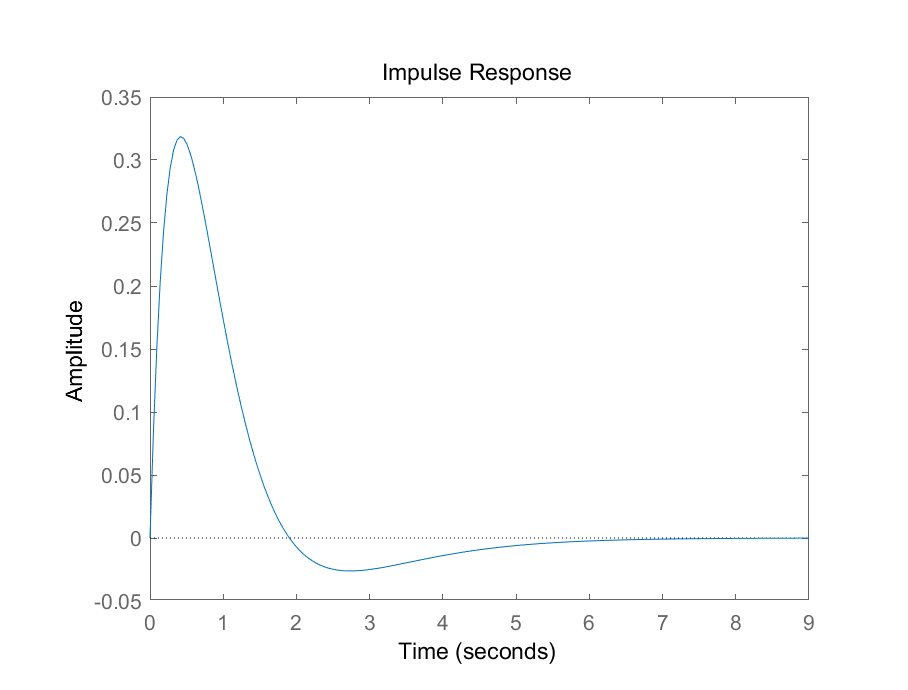
\includegraphics[width=0.6\textwidth]{1(b)-2.eps}
    \end{center}
    \caption{1(b)-2.}
\end{figure}

2. (a) The sketches of $X_p(\omega)$ for $-9\pi\leq\omega\leq9\pi$ for $\omega_0=\pi,\ 2\pi,\ 3\pi,\ \text{and}\ 5\pi$ are respectively
\begin{figure}[H]
    \begin{center}
        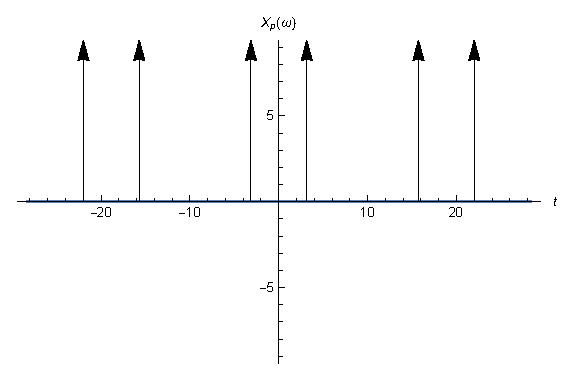
\includegraphics[width=0.6\textwidth]{2(a)i.eps}
    \end{center}
    \caption{2(a)i.}
\end{figure}
\begin{figure}[H]
    \begin{center}
        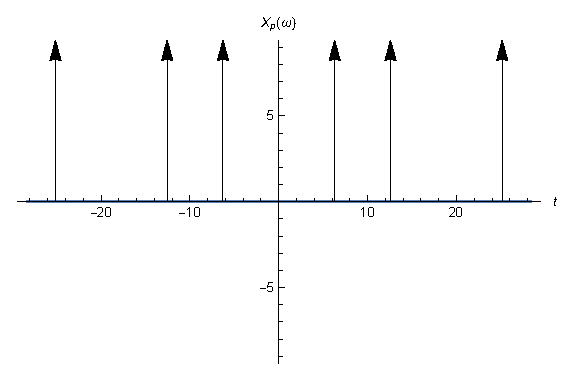
\includegraphics[width=0.6\textwidth]{2(a)ii.eps}
    \end{center}
    \caption{2(a)ii.}
\end{figure}
\begin{figure}[H]
    \begin{center}
        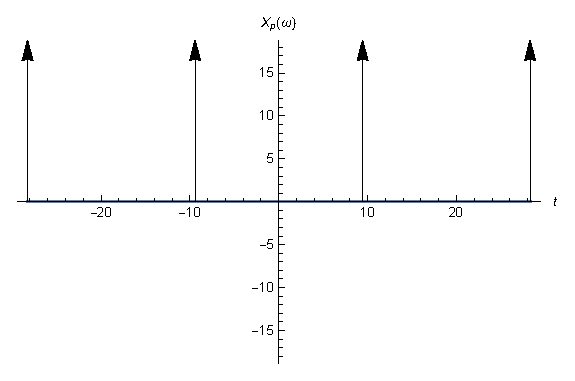
\includegraphics[width=0.6\textwidth]{2(a)iii.eps}
    \end{center}
    \caption{2(a)iii.}
\end{figure}
\begin{figure}[H]
    \begin{center}
        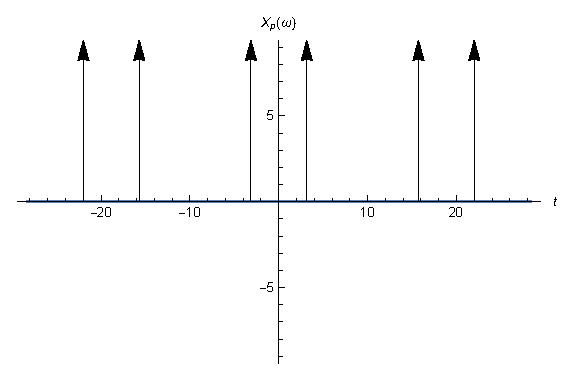
\includegraphics[width=0.6\textwidth]{2(a)iv.eps}
    \end{center}
    \caption{2(a)iv.}
\end{figure}

11. (b) The sketch of the efficiency of the modulated signal as a function of the modulated index $m$ is
\begin{figure}[H]
    \begin{center}
        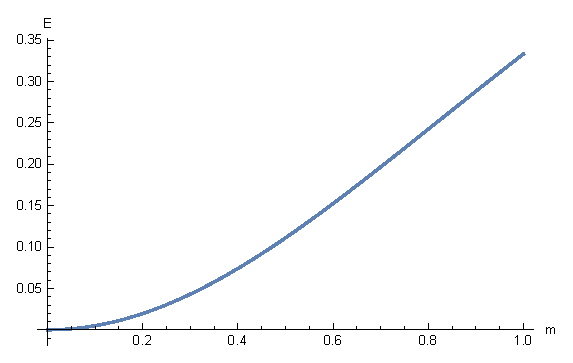
\includegraphics[width=0.6\textwidth]{11(b).eps}
    \end{center}
    \caption{11(b).}
\end{figure}
\end{document}